\setcounter{equation}0

\def\ryse{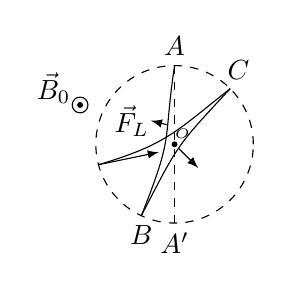
\begin{tikzpicture}
    \draw[dashed](0,0) circle (1);
\draw[fill=black](0,0) circle (.03);
\draw[dashed](90:1)--(270:1);
\draw(45:1) .. controls (0,-.05) and (.05,0) .. (245:1);
\draw[-latex](.05,-.05)--(.3,-.3);
\draw(45:1) .. controls (0,.15) and (-.1,0) .. (195:1);
\draw[-latex](195:1)--(-.2,-.1);
\draw(245:1) .. controls (0,.15) and (-.15,0) .. (90:1);
\draw[-latex](-.1,.25)--(-.3,.3);
  \begin{scope}[xshift=-1.2cm,yshift=.5cm]
\node[left,yshift=6] at(0,0){$\vec B_{0}$};
\draw(0,0) circle (.1);
\draw[fill=black](0,0) circle (.03);
\end{scope}
\node[left] at(-.2,.3){$\vec F_{L}$};
\node at(.1,.13){\tiny$O$};
\node[below] at(245:1){$B$};
\node[below] at(270:1){$A'$};
\node[above] at(90:1){$A$};
\node[above=-.05,xshift=3] at(45:1){$C$};
\end{tikzpicture}}


\def\rysd{\begin{tikzpicture}
\tkzDefPoint(30:1){v}
\tkzDefPoint(-60:.8){f}
\tkzDefPoints{0/0/o,1.7/0/x,0/-.7/y}
\draw(0,0) circle (.15);
\draw[fill=black](0,0) circle (.03);
\draw[->](-.7,0)--(1.5,0);
\draw[->](0,-.7)--(0,1.5);
\draw[-latex](o)--(v);
\draw[-latex](o)--(f);
\tkzDrawArc[black,R with nodes](o,.6)(x,v)
\tkzDrawArc[black,R with nodes](o,.6)(y,f)
\node[left,yshift=6] at(o){$B_{0}$};
\node[left] at(0,1.4){$y$};
\node[below=.05] at(1.4,0){$x$};
\node[above] at(v){$v$};
\node[right] at(f){$F_{L}$};
\node at(.1,-.45){$\beta$};
\node at(.45,.1){$\beta$};
\end{tikzpicture}}


\def\rysb{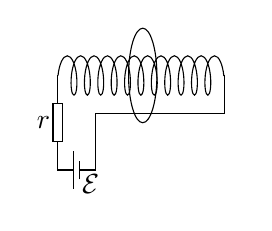
\begin{tikzpicture}[scale=1.2]
\node (a) at (0,0) {};
\node (b) at (1.97,0) {};
\draw[decoration={aspect=0.3, segment length=1.7mm, amplitude=2.5mm,coil},decorate] (a) -- (b);
\draw[thin](.1,0)--(.1,-1)--(.5,-1)--(.5,-.4)--(1.865,-.4)--(1.865,0);
\draw[fill=white](.05,-.7) rectangle (.15,-.3);
\draw[white](.27,-1)--(.33,-1);
\draw(.27,-1.2)--(.27,-.8);
\draw(.33,-1.1)--(.33,-.9);
\node at(-.05,-.5){$r$};
\node at(.45,-1.15){$\mathcal E$};
\draw(1,0) ellipse (.15 and .5);
\end{tikzpicture}}


\def\rysa{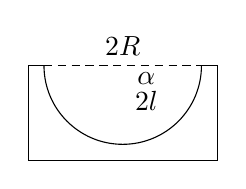
\begin{tikzpicture}
  \draw
    (0,0) arc(180:360:1)
    ;
    \draw(0,0)--(-.2,0)--(-.2,-1.2)--(2.2,-1.2)--(2.2,0)--(2,0);
    \draw[densely dashed](0,0)--(2,0);
    \tkzDefPoint(220:1){a}
    \tkzDefShiftPoint[a](1,0){aa}
    \tkzDefPoint(2,0){b}
    \tkzDefPoint(1,0){o}
        \tkzDrawLines[very thick,add=0 and .3](aa,b);
        \tkzDrawArc[black,R with nodes](b,.9)(o,aa)
        \node[above] at(1,0){$2R$};
        \node at(1.3,-.45){$2l$};
        \node[below] at(1.3,.04){$\alpha$};
\end{tikzpicture}}


\def\ryslfa{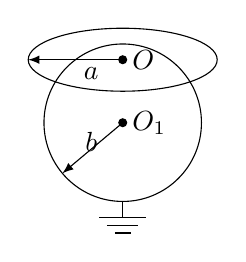
\begin{tikzpicture}[black]
  \draw(0,0) circle(1);
  \draw[fill](0,0) circle(.05);
  \draw[fill](0,.8) circle(.05);
  \draw(0,.8) ellipse(1.2 and .4);
  \draw[-latex](0,.8)--(-1.2,.8);
  \draw[-latex](0,0)--(220:1);
  \node[right] at(0,0){$O_{1}$};
  \node[right] at(0,.8){$O$};
  \node[below] at(-.4,.83){$a$};
  \node[below] at(-.4,0){$b$};
  \draw(0,-1)--(0,-1.2);
  \draw(-.3,-1.2)--(.3,-1.2);
  \draw(-.2,-1.3)--(.2,-1.3);
  \draw(-.1,-1.4)--(.1,-1.4);
\end{tikzpicture}}
\def\sqqrt#1{\sqrt{\vphantom{b}\smash{#1}}}
\def\ora#1{\overrightarrow{#1}}
\def\e{{\rm{e}}}
\def\F{{\cal F}}
\def\R{{\mathbb R}}
\def\Q{{\bf Q}}
\def\N{{\bf N}}
\def\Z{{\bf Z}}
%\def\pp{{\bf p}}
%\def\qq{{\bf q}}
%\def\ss{{\bf s}}
\def\vv{{\bf v}}
\def\bb{{\bf b}}
\def\xx{{\bf x}}
%\def\yy{{\bf y}}
%\def\zz{{\bf z}}
\def\tg{{\rm{tg}\,}}
\def\ctg{{\rm{ctg}\,}}
\def\arctg{{\rm{arc\,tg}\,}}
\def\arcctg{{\rm{arc\,ctg}\,}}
%\def\bdot{\mathop{\lower-2pt\hbox{\bf.}}}
%\def\"{\hbox to.2em{},\kern-.5em\hbox{,}\hbox to.3em{}}
%\def\nlss{\noalign{\smallskip}}
\def\frac#1#2{{#1\over#2}}
\def\xleft#1\right{#1}

\let\arcangle\angle
\long\def\nic#1{}


\setcounter{equation}0
\normalsize

\makeatletter
 \def\@oddhead{\hbox to\hsize{\kern-7.5cm\rlap{\color{magenta!20}{\vrule height.9cm depth-1mm width22.5cm}}\kern2cm{\textcolor{white}{\LARGE\raise3mm\hbox{\textsf{\textbf{Liga zadaniowa Wydziału Matematyki, Informatyki i~Mechaniki,}}}}\hfill}\hfill\kern-3cm}}
\makeatother

% LIGA--MATEMATYCZNA--ZDEFINIOWANIE
\ligaspis
\long\def\matematyka{ 
%\vspace{-30pt}
\klub[3]{m}
  \Magenta{\textbf{Zadania z~matematyki nr 893, 894}}%
  \marg{Termin nadsyłania rozwiązań: \rlap{31 III~2025}
    \vskip1cm
    
    {\centering
Czołówka ligi zadaniowej {\bf Klub 44~M}\\
po uwzględnieniu ocen rozwiązań zadań\\[1pt]
 883 ($WT = 1{,}82$) i~884 ($WT = 1{,}61$)\\
z~numeru 6/2024
\vskip2pt}\tabcolsep5.5pt
\tabcolsep3pt
\begin{tabular}{@{}llr}

Michał Adamaszek&Kopenhaga &46,32\\
Szymon Kitowski&Warszawa &41,11\\
Witold Bednarek&Łódź &40,58\\
Mikołaj Pater&      &39,58\\
Krzysztof Zygan&Lubin &39,38\\
Andrzej Daniluk&Warszawa &37,89\\
Tomasz Wietecha&Tarnów &35,18\\
Andrzej Kurach&Ryjewo &33,24\\
Jędrzej Biedrzycki&    &32,29\\
  Krzysztof Kamiński&Pabianice &30,48\\
  \end{tabular}
\medskip


Pan Michał Adamaszek, autor wielu znakomitych zadań -- teraz już
Weteran do kwadratu: trzykroć trzy razy czterdzieści cztery!

}

 \Black{\textit{Redaguje Marcin E. KUCZMA}}

\advance\baselineskip by-.2pt
{\bf893.}
Punkty $A,B,C,D,E$ leżą w~tym porządku na linii prostej, przy czym ${CA=CE}$, ${CB=CD}$. Poza tą prostą, po jednej jej stronie, leżą punkty $K$ i~$L$ takie, że trójkąty $AKB$ i~$DLE$ mają ostre kąty przy wierzchołkach $A,B$ i~$D,E$, a~suma miar tych czterech ostrych kątów wynosi~$180^\circ$. Proste $KB$ i~$LD$ przecinają się w~punkcie~$N$; proste $AK$ i~$EL$ przecinają się w~punkcie~$M$; punkty $M,N$ leżą po różnych stronach prostej $KL$, a~ponadto ${MN\perp{AE}}$. Dowieść, że ${CK=CL}$.


{\bf894.}
Wyznaczyć wszystkie trójki liczb całkowitych $(x,y,z)$ spełniające równanie
$$
\frac{x+y+xyz}{yz+1}=\frac{2025}{44}\,.
$$

{\em Zadanie 894 zaproponował pan Paweł Kubit z Krakowa.}

%\vspace*{\parskip}
%\begin{dwieszpalty}
{\Magenta{\textbf{Rozwiązania zadań z~numeru 9\slash2024}

{\footnotesize Przypominamy treść zadań:}

{\scriptsize\advance\baselineskip by-.3pt
{\bf885.}
Niech $p$ będzie ustaloną liczbą pierwszą nieparzystą i~niech ${M=\{1,2,\ldots,p{-}1\}}$. Wyznaczyć liczbę funkcji ${f\colon\,M\to{M}}$ takich, że dla każdego ${x\in{M}}$ liczba $\,{xf(f(x))-1}\,$ dzieli się przez~$p$.


{\bf886.}
W~trójkącie ostrokątnym o~bokach długości $a,b,c$ kąty wewnętrzne przy przeciwległych wierzchołkach mają miary (odpowiednio) $\alpha,\beta,\gamma$. Wykazać, że wartość ilorazu
$$
\frac{a\,\cos\alpha+b\,\cos\beta+c\,\cos\gamma}{a+b+c}
$$
wyraża się przez długości promieni okręgów opisanego i~wpisanego. Wyjaśnić, czy uzyskany wzór jest słuszny również dla trójkątów rozwartokątnych.



}
}}


\begin{dwieszpalty}\advance\parskip by-2pt\footnotesize\advance\baselineskip by-.2pt
{\bf885.}
Każdy element ${x\in{M}}$ ma w~zbiorze~$M$ dokładnie jeden element odwrotny (mod~$p$), który będziemy oznaczać~$x^{-1}$; tj.~taki, że ${xx^{-1}\equiv1}$~(mod~$p$). Dany w~zadaniu warunek przepisujemy jako równanie
$$
ff(x)=x^{-1}\quad\ \hbox{dla wszystkich}\ x\in{M}
\leqno(1)
$$%
\looseness-1 {\spaceskip.33em minus.17em(notacja ,,oszczędna'': ${f\circ{f}=ff}$). Gdy funkcja~$f$ spełnia równanie~(1), wówczas ${ffff(x)=x}$, skąd wniosek, że $f$ jest bijekcją zbioru~$M$ na~$M$ -- czyli jest permutacją zbioru~$M$ -- który wobec tego rozpada się na rozłączne cykle tej permutacji. Skoro $ffff$ jest identycznością, długość cyklu może wynosić jedynie 1,~2 lub~4.}

Gdy $x$ wchodzi do cyklu długości 1 lub~2, to ${ff(x)=x}$, więc zgodnie z~(1) ${x=x^{-1}}$, co oznacza, że ${x=1}$ lub ${x=p{-}1}$. Działanie funkcji~$f$ w~obrębie zbioru $\{1,p{-}1\}$ może mieć jedną z~dwóch postaci:
$$
[\,1\mapsto1,\;p{-}1\mapsto p{-}1\,]
 \quad
    \hbox{lub}\quad
[\,1\mapsto p{-}1\mapsto1\,].
  \leqno(2)
$$%
Pozostała część zbioru~$M$, czyli zbiór ${L=\{2,\ldots,p{-}2\}}$ musi być już sumą cykli długości~4. Tak więc ${p\equiv3}$~(mod~4); dla ${p\equiv1}$~(mod~4) nie istnieje ani jedna funkcja~$f$ o~badanej własności.

Dalej przyjmijmy, że ${p=4n+3}$ (dla pewnego ${n\in\N}$); więc $L$ to suma $n$~cykli długości~4.

Z~każdej pary $\{x,x^{-1}\}$ wybierzmy jeden element -- np.~mniejszą liczbę. Wybrane elementy utworzą zbiór (mocy~$2n$), który nazwiemy~$K$ (przykładowo, dla ${p=11}$ zbiór ${K=\{2,3,5,7\}}$). Każdy \hbox{4-cykl} zawiera dwa elementy ${a,b\in{K}}$ oraz ich odwrotności; przy tym działanie~$f$  w~takiej czwórce ma jedną z~dwóch postaci:
$$%\begin{aligned}
[\,a\mapsto{b}\mapsto{a^{-1}}\mapsto{b^{-1}}\mapsto{a}\,]
\
    \hbox{lub}\
[\,a\mapsto{b^{-1}}\mapsto{a^{-1}}\mapsto{b}\mapsto{a}\,].
%  \end{aligned}
  \leqno(3)
$$%
Możliwe rozbicia zbioru~$L$ na $n$ dopuszczalnych czwórek odpowiadają rozbiciom~$K$ na $n$ par $\{a,b\}$. Jest ${(2n-1)!!}$ takich rozbić. [Uzasadnienie: bierzemy najmniejszą liczbę ${a\in{K}}$ i~łączymy ją w~parę z~dowolnym innym elementem ${b\in{K}}$ (${2n-1}$~możliwości); bierzemy najmniejszą liczbę różną od~$a$,~$b$ i~łączymy ją
w~parę z~dowolnym niewykorzystanym elementem (${2n-3}$~możliwości)~itd.]. Uzyskaną wartość mnożymy przez~$2^n$ (by uwzględnić swobodę wyboru jednej z~opcji~(3) w~każdej z~$n$~czwórek). To daje liczbę dopuszczalnych permutacji w~obrębie zbioru~$L$. Jeszcze jedno pomnożenie przez~2 (uwzględniające wybór~(2) w~zbiorze $\{1,p{-}1\}$) daje ostateczny wynik: liczba funkcji~$f$, o~jakie pyta zadanie, wynosi~0, gdy $p$ ma postać ${4k+1}$, oraz ${2^{n+1}(2n-1)!!}$, gdy ${p=4n+3}$.


{\bf886.}
Gdy trójkąt $ABC$ jest ostrokątny, środek~$O$ okręgu opisanego leży wewnątrz niego. Odległości punktu~$O$ od boków $a,b,c$ oznaczmy przez $d_a$,~$d_b$,~$d_c$. W~trójkącie $OBC$ (równoramiennym) ${d_a=R\cos\alpha}$ jest wysokością, a~jego pole wynosi $\frac12ad_a$. Analogicznie wyrażają się pola trójkątów $OCA$ i~$OAB$; suma tych trzech pól to pole trójkąta~$ABC$, wyrażające się też jako iloczyn ${\frac12(a+b+c)r}$ \ ($R$~i~$r$ to promienie okręgów opisanego i~wpisanego). Zatem
$$
\textstyle
\frac12aR\cos\alpha+\frac12bR\cos\beta+\frac12cR\cos\gamma=\frac12(a+b+c)r,$${czyli}
$$\displaystyle
\frac{a\cos\alpha+b\cos\beta+c\cos\gamma}{a+b+c}=\frac{r}R\,.
$$
Ten wzór jest nadal słuszny, gdy trójkąt $ABC$ jest rozwartokątny; np. ${\alpha>90^\circ}$. Wtedy ${\cos \alpha<0}$, odległość~$d_a$ równa jest nie $R\cos \alpha$, lecz $-R\cos \alpha$; ale też trójkąt $OBC$ leży na zewnątrz trójkąta $ABC$ i~jego pole należy odjąć od sumy pól trójkątów $OCA$,~$OAB$, obliczając pole~$ABC$. Minusy się redukują, wynik ${{r}\slash{R}}$ pozostaje w~mocy. [Można było od razu na starcie określić~$d_a$ jako odległość opatrzoną znakiem ({\it signed distance}), wtedy rozważanie przypadków staje się zbędne].

\end{dwieszpalty}



\normalsize
}

% -------------------- LIGA--FIZYCZNA--ZDEFINIOWANIE ---------------------------------------

\long\def\fizyka
{\klub[5]{f}  
\Magenta{\textbf{Zadania z~fizyki nr 790, 791}}%
\marg{Termin nadsyłania rozwiązań: \rlap{31 III 2025}\medskip}
% \baselineskip11.9pt plus.3pt minus.2pt 

\Black{\textit{Redaguje Elżbieta ZAWISTOWSKA}}%

{\bf 790.} Jednorodny pręt o~długości $2l$ opiera się na krawędzi nieruchomej, półkolistej czaszy o~promieniu $R$ (rys. 1). Jaki kąt $\alpha$  tworzy pręt z~płaszczyzną poziomą w~położeniu równowagi? Tarcie zaniedbujemy.

{\bf 791.} O~jaką wielkość zmieni się natężenie prądu w~kołowej pętli z~nadprzewodnika, gdy nałożymy ją na długą zwojnicę podłączoną do baterii o~sile elektromotorycznej $\mathcal E$ (rys.~2). Całkowity opór obwodu ze zwojnicą wynosi~$r$, liczba zwojów~$N$, współczynnik samoindukcji zwojnicy~$L_{0}$, a~pętli~$L$. Indukcję wzajemną zaniedbujemy.
\marg{\rysa\\[4pt]
  Rys. 1
  
\rysb\\[4pt]
Rys. 2


  





}
\marg[-155]{
   \nic
  {{\centering
Czołówka ligi zadaniowej {\bf Klub 44~F}\\
po uwzględnieniu ocen rozwiązań zadań\\
778 ($WT=1{,}95$), 779 ($WT=3{,}15$) z~numeru 5/2024
\vskip2pt}
\tabcolsep3pt
\begin{tabular}{@{}l@{}l@{}r}
  Paweł Perkowski            &Ożarów Maz.            &5--43,19\\
Jacek Konieczny              &Poznań                            &40,87\\
Konrad Kapcia                 &Poznań                      &2--39,97\\
Tomasz Wietecha           &Tarnów                   &17--30,38\\
Andrzej Nowogrodzki\!\\&Chocianów               &3--27,19\\
  Jan Zambrzycki                &Białystok                  &4--25,85\\
  \end{tabular}

\medskip

%Termin nadsyłania rozwiązań: \rlap{28 II~2025}
\medskip


}
}


{\Magenta{\textbf{Rozwiązania zadań z~numeru 9\slash2024}

{\footnotesize Przypominamy treść zadań:}\medskip
 
{\scriptsize 
  \hbox to\hsize{\vbox{\hsize9.5cm{\bf 782.} Potencjał w~środku odosobnionego, naładowanego, drucianego pierścienia o~promieniu~$a$ wynosi $\varphi_{O}$. Pierścień ten zbliżono do uziemionej przewodzącej sfery o~promieniu $b$ tak, że tylko środek pierścienia znajduje się na powierzchni sfery (rys.~3). Znaleźć ładunek indukowany na sferze.

{\bf 783.} Mała kulka o~masie $m$ naładowana ładunkiem $q$ zawieszona jest na nieważkiej i~nierozciągliwej nici w~jednorodnym polu magnetycznym o~indukcji~$B_{0}$ skierowanej pionowo. Kulkę odchylono o~mały kąt z~położenia równowagi i~puszczono swobodnie. Po jakim czasie płaszczyzna wahań wahadła obróci się o~kąt~$2\pi$? Maksymalna siła Lorentza działająca na kulkę jest mała w~porównaniu z~maksymalną siłą zawracającą. Nie uwzględniamy efektów związanych z~obrotem Ziemi.
}\hfill  \begin{tabular}[b]{@{}l@{}}\ryslfa\\ \textcolor{black}{Rys. 3}
         \end{tabular}}}
     
}
}

\begin{dwieszpalty}\footnotesize
\textbf{782.}
Potencjał w~środku odosobnionego pierścienia jest równy
$\varphi _O=\sum_i{{kq_i}/{a}}={kQ/a}$,  stąd ładunek pierścienia $Q=\nobreak {a{\varphi }_O}/{k.}$
 Potencjał uziemionej sfery oraz w~jej wnętrzu wynosi zero i~pochodzi od naładowanego pierścienia oraz ładunków indukowanych na sferze. Ładunki indukowane nie są rozłożone równomiernie, dlatego najłatwiej jest wyrazić potencjał w~środku sfery:
\[0=k{Q}/{\sqrt{a^2+b^2}}+k{Q_{\rm ind}}/{b.}\] 
Szukany ładunek indukowany dany jest wzorem:
\[Q_{\rm ind}=-Q{b}/{k\sqrt{a^2+b^2}}=-4\pi {\varepsilon }_0ab{{\varphi }_O}/{\sqrt{a^2+b^2.}}\]


\textbf{783.}
Będziemy zakładać, że ładunek $q$ jest dodatni, a~pole magnetyczne skierowane w~górę. Wprowadźmy układ współrzędnych, którego początek umieszczamy w~punkcie zawieszenia, oś $z$ skierowana jest pionowo w~górę, a~osie $x$ i $y$ leżą w~płaszczyźnie poziomej. Równanie ruchu kulki ma postać:
\[m\boldsymbol{a}=m\boldsymbol{g}+\boldsymbol{T}+{\boldsymbol{F}}_L,\] 
gdzie $\boldsymbol{a}={d^2\boldsymbol{r}}/{dt^2}$,  $\boldsymbol{r}=(x,y,z)$ jest wektorem położenia kulki, $\left|\boldsymbol{r}\right|=l$ jest długością wahadła, siła naprężenia nici $\boldsymbol{T}=-T{\boldsymbol{r}}/{l}$. Dla małych drgań $T\cong mg$. W~tym przybliżeniu kulka porusza się praktycznie w~płaszczyźnie poziomej, a~składowe siły Lorentza wynoszą (rys.~4):
\[F_{Lx}=F_L\sin \beta =qv_yB_0,  F_{Ly}=-F_L\cos \beta =-qv_xB_0,  F_{Lz}=0.\] 
Równanie ruchu w~rzucie na osie $x,y$ ma postać:
\begin{equation} \label{GrindEQ__1_} 
ma_x=-mg{x}/{l}+qv_yB_0,        ma_y=-mg{y}/{l}-qv_xB_0. 
\end{equation} 
W~nieobecności pola magnetycznego wahadło wykonuje drgania w~jednej płaszczyźnie z~częstością ${\omega }_0=\sqrt{{g}/{l}}$. Gdy pole $B_0\neq 0$, siła Lorentza zakrzywia tor kulki, ale ponieważ nie wykonuje pracy, maksymalne wychylenie nici z~położenia równowagi pozostaje stałe. Z~zasady zachowania energii
\[\thickmuskip2mu\frac{m{(v_{\max})}^2}{2}=mgl\left(1-\cos \alpha _{\max}\right)=2mgl\sin^2\left(\frac{{\alpha }_{\max}}{2}\right)=\frac{mgl{\left({\alpha }_{\max}\right)}^2}{2},\] 
\[v_{\max}={\alpha }_{\max}\sqrt{gl.}\] 
Ponieważ maksymalna siła Lorentza jest mała w~porównaniu z~maksymalną siłą zawracającą ${F_Z}_{\max}$,
\[\frac{{F_L}_{\max}}{{F_Z}_{\max}}=\frac{qB_0v_{\max}}{mg{\alpha }_{\max}}=\frac{qB_0}{m}\sqrt{\frac{l}{g}}=\frac{{\omega }_B}{{\omega }_0}\ll 1,\] 
gdzie ${\omega }_B={qB_0}/{m}$ jest częstością ruchu obrotowego cząstki naładowanej, poruszającej się po okręgu w~jednorodnym polu magnetycznym. W~czasie półokresu drgań pole magnetyczne w~niewielkim stopniu zakrzywia trajektorię kulki.

Korzystając z~wprowadzonych oznaczeń, możemy przepisać równania \eqref{GrindEQ__1_} w~postaci:
\begin{equation} \label{GrindEQ__2_} 
{d^2x}/{dt^2}=-{{\omega }_0}^2x+{\omega }_B{dy}/{dt},  \quad      {d^2y}/{dt^2}=-{{\omega }_0}^2y-{\omega }_B{dx}/{dt}. 
\end{equation} 
Równania \eqref{GrindEQ__2_} są równaniami liniowymi, obowiązuje więc zasada superpozycji -- dowolna kombinacja liniowa dwóch rozwiązań tych równań jest też rozwiązaniem.



Gdy nie ma pola magnetycznego, równania \eqref{GrindEQ__2_} są niezwiązane. Dwa rozwiązania opisujące drgania w~płaszczyznach $xz$ i $yz$ mają postać:
\begin{equation}
  \label{GrindEQ__3_}x_1=A\cos \omega t,\  y_1=0\text{  oraz  }x_2=0,\  y_2=A\sin\omega t,\text{   gdzie }\omega ={\omega }_0.
\end{equation}
Dodając i~odejmując stronami te rozwiązania, otrzymujemy rozwiązania opisujące ruchy wahadła stożkowego w~kierunkach przeciwnym i~zgodnym ze wskazówkami zegara:
\begin{equation} \label{GrindEQ__4_} \begin{aligned}
                       &
x_3=x_1+x_2=A\cos \omega t,\  y_3=y_1+y_2=A\sin \omega t;\\& x_4=A\cos \omega t,\  y_4=-A\sin\omega t 
                                     \end{aligned}
                                   \end{equation} 
i~odwrotnie $x_1={\left(x_3+x_4\right)}/{2}$.

W~przypadku $B_0\neq 0$ rozwiązania \eqref{GrindEQ__3_} nie spełniają już równań \eqref{GrindEQ__2_}, natomiast  rozwiązania \eqref{GrindEQ__4_}  spełniają je, gdy ${\omega }^2={{\omega }_0}^2-{\omega }_B\omega $, stąd
\[\omega =-{{\omega }_B}/{2}\pm \sqrt{{{\omega }_0}^2+{{{\omega }_B}^2}/{4}}\cong -{{\omega }_B}/{2}\pm {\omega }_0.\] 
Zgodnie z~zasadą superpozycji równania \eqref{GrindEQ__2_} spełniają również rozwiązania:
\begin{align*}
  x&=\frac{\left(x_3+x_4\right)}{2}=A\left[\cos \left({\omega }_0+\frac{{\omega }_B}{2}\right)+\cos \left({\omega }_0-\frac{{\omega }_B}{2}\right)\right]\\&=A\cos {\omega }_0\cos \left(\frac{{\omega }_B}{2}\right),\\
y&=\frac{\left(y_3+y_4\right)}{2}=A\sin {\omega }_0\sin \left(\frac{{\omega }_B}{2}\right).
\end{align*}
Równania opisują drgania wahadła z~częstością ${\omega }_0$ w~płaszczyźnie, która sama obraca się z~częstością ${{\omega }_B}/{2}$. Tor kulki w~płaszczyźnie~$xy\ $ ilustruje rys.~5.

Szukany czas obrotu płaszczyzny wahań o~kąt 2$\pi $ wynosi:
\[t={4\pi }/{{\omega }_B}={4\pi m}/{\left|qB_0\right|}.\] 
{
  \scriptsize
  Rys. 4\rysd
\hskip2cm
  Rys. 5\kern-.5cm
\ryse

}\end{dwieszpalty}
}


\makeatletter
%\def\@oddhead{\vbox to0pt{\hbox to\hsize{\kern-7.5cm\rlap{\color{magenta!20}{\vrule height.9cm depth-1mm width22.5cm}}\kern2cm{\textcolor{white}{\LARGE\raise3mm\hbox{\textsf{\textbf{Liga zadaniowa Wydziału Matematyki, Informatyki i~Mechaniki,}}}}\hfill}\hfill\kern-3cm}\vspace{-4pt}
%  \hbox to\hsize{\kern-7.5cm\rlap{\color{magenta!20}{\vrule height.9cm depth-1mm width22.5cm}}\kern2cm{\textcolor{white}{\LARGE\raise3mm\hbox{\textsf{\textbf{Wydziału Fizyki Uniwersytetu Warszawskiego i~Redakcji \textit{Delty}}}}}\hfill}\hfill\kern-3cm}\vss}}
%\def\@oddhead{\vbox{\hbox to\hsize{\kern-7.5cm\rlap{\color{magenta!20}{\vrule height.9cm depth-1mm width22.5cm}}\kern2cm{\textcolor{white}{\LARGE\raise3mm\hbox{\textsf{\textbf{Liga zadaniowa Wydziału Matematyki, Informatyki i~Mechaniki,}}}}\hfill}\hfill\kern-3cm}\vspace{-4pt}
% \hbox to\hsize{\kern-7.5cm\rlap{\color{magenta!20}{\vrule height.9cm depth-1mm width22.5cm}}\kern2cm{\textcolor{white}{\LARGE\raise3mm\hbox{\textsf{\textbf{Wydziału Fizyki Uniwersytetu Warszawskiego i~Redakcji \textit{Delty}}}}}\hfill}\hfill\kern-3cm}}}
\makeatother
  
\normalsize

%\vspace*{0pt}

\fizyka

\makeatletter
 \def\@oddhead{\hbox to\hsize{\kern-7.5cm\rlap{\color{magenta!20}{\vrule height.9cm depth-1mm width22.5cm}}\kern2cm{\textcolor{white}{\LARGE\raise3mm\hbox{\textsf{\textbf{Wydziału Fizyki Uniwersytetu Warszawskiego i~Redakcji \textit{Delty}}}}}\hfill}\hfill\kern-3cm}}
\makeatother

\normalsize
\bigskip\matematyka

%\vskip-14pt
\regulamin



\normalsize

%\hspace*{-5.5cm}\vrule height1pt width18cm

\vfill\eject\setcounter{equation}0
\makeatletter
\def\@oddhead{\hfill}
\makeatother
\normalsize

